\documentclass{article}
\usepackage{gensymb}
\usepackage[backend=biber]{biblatex}
\usepackage{graphicx}
\usepackage[colorlinks=true]{hyperref}
\usepackage{booktabs}
\usepackage{siunitx}
\usepackage[]{amsmath}
\usepackage{mathtools}
\usepackage{fancyref}
\usepackage{fancyheadings}
\usepackage{lipsum}
\addbibresource{/Users/giorgio/Bibliography/bibliography.bib}
\hypersetup{
    colorlinks=true,
    linkcolor=blue,
    filecolor=magenta,  
    citecolor=blue,    
    urlcolor=cyan,
    pdftitle={Selective Laser Sintering for sustainable polymers},
    bookmarks=true,
}

\author{Giorgio De Trane, s275514}
\title{\textbf{Selective Laser Sintering for sustainable polymers}}

\begin{document}
    \setlength{\parindent}{0pt}
    \maketitle
    \begin{center}
        
\includegraphics[width=0.8\textwidth]{Pictures/polito_logo.eps}\linebreak\newline
        
        \textit{Year 2021/2022}
    \end{center}

    \newpage
    \begin{center}
        To my parents, whose love has always been unconditional, intense and at times hard to comprehend. 
    \end{center}
    \newpage

    \begin{abstract}
        The goal of this case study is to optimize the production of SLS suitable fine powders of sustainable biopolymers. 

        After an extensive research on current \textit{state-of-the-art} production methods, suitable processes have been experimented, 
        with the available lab equipment, leading to the choice of \textit{chemical precipitation}. 

        An initial recipe for \textit{PHBH}, previously tested by other researchers at \textit{DISAT, PoliTo}, has been tweaked and improved, 
        achieving over a ten-fold increase in pellet-to-powder production yield. 

    \end{abstract}
    \newpage
    \tableofcontents
    \newpage 
    \listoffigures
    \newpage
    %\listoftables
    \newpage
    \section{Introduction\label{Intro}}

    \textit{Additive manufacturing} (AM) is a broad term that encompasses several manufacturing techniques, characterized by their additive nature, as the name suggests, 
    in contrast with more traditional subtractive processes.
    
    AM techniques are applied to a vast range of materials, including ceramics, polymers and metal alloys, some of which are specifically developed or optimized to 
    these kinds of applications. \\ 
    
    The main advantage of AM is the ability to produce complex shapes in a relatively short time. 
    These geometries are either too hard or even impossible to reproduce with subtractive manufacturing techniques, which often require multiple steps, using different 
    pieces of equipment, trained personnel, etc. \\

    Given the same material, the complex shapes allowed by AM can replace components made of multiple assembled parts with a unique solid piece of comparable or even better mechanical properties. 
    
    The inherent flexibility of AM often allows product designers to simplify or even entirely bypass the very strict CAD workflow (which is inherently tied to 
    traditional manufacturing processes) and make use of organic and/or generative modeling. 

    As a consequence of better design choices and minimal need of post-processing of AM objects, far less raw material is wasted, compared to subtractive manufacturing techniques, leading to 
    long term lowering of costs, faster design-to-market pipelines and, last but not least, lower emissions and environmental impact \autocite*{Recent_progress_polymers_AM}. 

    \subsection{Polymers in Additive Manufacturing\label{Polymers_in_AM}}

    Polymers and their composite materials have been used in all sorts of fields, ranging from arts and crafts all the way to advanced biomedical and aerospace applications, thanks 
    to their unique and varied extended range of properties. \\  
    
    The rapid advancement of AM, where polymers have been extensively used for prototyping, in the form of resins, filaments, powders and viscous inks, 
    has increased the demand for high-performance polymers, in order to take advantage of their quicker printing times (compared to metals) as well as their lower cost, while still
    maintaining good mechanical properties for an end product, rather than just a prototype \autocite*{Recent_progress_polymers_AM}. \\ 

    The urge for drastically reducing the environmental impact of human activities involves every production field, including AM, which can be inherently less impactful
    than traditional manufacturing processes, given the same material and final product to achieve. 

    A consequence of the concerns about climate change and its potentially catastrophic outcomes is the research in the field of eco-friendly materials, including polymers 
    that could be used in AM. 
    
    A great example is \textit{PLA} (PolyLactic Acid), a polymer widely used in 3D printing, whose monomer is obtained by fermenting starches, such as corn starch. \\ 

    Many new eco-friendly polymers have been and are currently being studied for AM techniques, but this case study will focus mostly on materials that can be potentially turned 
    into powders for \textit{PBF} (Powder Bed Fusion) techniques or filaments for \textit{ME} (Material Extrusion). 
    
    \subsection{Common AM techniques for polymers\label{AM_techniques_summary}}
    
    Polymers can be processed with several AM techniques, including, but not limited to: 

    \begin{itemize}
        \item \textbf{VP} (Vat Photopolymerization), which makes use of UV lights (or other radiations) to solidify photosensitive resins. This class of AM processes can produce 
                        parts with the highest resolution among all AM methods \autocites*{Recent_progress_polymers_AM}{Kovalcik_PHA_Review};
        \item \textbf{MJ} (Material Jetting), which consist of a deposition of viscous fluids (either in droplets or in a continuous fashion), solidified by different agents 
                            (time interacting chemicals, heating, cooling, drying, photopolymerization, etc.). These processes include several patented methods, characterized by 
                            high speed printing \autocite*{Recent_progress_polymers_AM};
        \item \textbf{PBF} (Powder Bed Fusion), where the object is printed by locally fusing a powder bed (with a pulsing energy source -such as lasers- or with a local deposition of chemicals),
                            layed out in a layer-by-layer fashion \autocites*{Recent_progress_polymers_AM}{Kovalcik_PHA_Review};
        \item \textbf{ME} (Material Extrusion), where each layer is printed by direct deposition of materials through a nozzle, that solidify as they cool down \autocites*{Recent_progress_polymers_AM}{Kovalcik_PHA_Review};
        \item \textbf{BJ} (Binder Jetting), similarly to 2D inkjet printing utilizes a
                        polymer in the form of a liquid binder, that gets deposited in droplets onto a powder bed (usually made of metallic or ceramic particles). This 
                        method can build large parts without support structures and the lack of a high power heat source cuts its cost down, but the structural 
                        properties of the final parts are poor compared to sintered equivalents, making heat treatments necessary \autocite*{Recent_progress_polymers_AM};
        \item \textbf{Sheet Lamination}, where thin sheets of material are stacked together and bonded with adhesives or heat. This class of techniques 
                        is not entirely additive, since subtractive processes are used to cut and refine the final part, creating substantial material waste \autocite*{Recent_progress_polymers_AM}.
    \end{itemize} \clearpage

    \subsubsection{FDM (Fused Deposition Modeling) \label{FDM_general}}

    FDM is a \textit{ME} technique and the most well known AM process, commonly named 3D printing in popular media. \\
    
    The process consists of a direct layer-by-layer deposition of a thermoplastic filament, heated up to its melting point (or enough to soften it until it reaches an 
    optimal flow) and extruded through a nozzle \autocites*{Recent_progress_polymers_AM}{Kovalcik_PHA_Review}. 

    The nozzle is generally moved in the x-y plane until a layer is completed with the desired infill, then either the extruder head or the growth plate are moved along the z axis, 
    initiating the printing of the subsequent layer.

    The planar infill and the resolution on the z axis will determine the quality of the final print for a given material and geometry, in terms of density and visual appeal.
    
    For a given planar infill, the z axis resolution greatly influences the final look of the part, as well as printing times:
    modern slicing software can analyze the geometry and generate an adaptive resolution, reducing the number of layers where the local  
    curvature of the object is within a certain threshold and increasing it when necessary. 
    
    This approach can produce good quality parts, 
    while reducing printing times. \\ 
    
    FDM has gained a lot of popularity in the last few years, given its general ease of use, relatively low cost of both materials and equipment and its growing 
    community of enthusiasts. \\

    A wide variety of materials can be used with this technique, including (but not limited to) 
    \textit{PLA}, \textit{ABS}, \textit{PET}, \textit{PETG}, \textit{HIPS}, \textit{TPU}, \textit{nylon}. \clearpage

    \subsubsection{SLS (Selective Laser Sintering) \label{SLS_general}}

    \textit{SLS} is a manufacturing process in the PBF family. 

    A powder bed is layed out onto a platform and a focused heat source (a laser) locally sinters the powder, 
    until a single layer is completed \autocites*{Recent_progress_polymers_AM}{Kovalcik_PHA_Review}. 

    A mechanism wipes out the remaining powder, which is recollected and automatically redistributed by a recoating 
    system, for each subsequent layer \autocite*{Padovano_SLS_Review}. 

    This process is similar to \textit{SLM} (Selective Laser Melting), typically used with metal alloys: in \textit{SLS} the energy input is not high enough 
    to bring the powders to their melting point, but sufficient for sintering of the powders. 

    Despite the slight difference, many sources use the terms interchangeably, often effectively referring to SLM in metal manufacturing. 
    
    When it comes to thermoplastic materials, the required laser power to sinter each layer is substantially lower than that needed for metals. \\ 

    \textit{SLS} printers can be considerably more expensive than \textit{FDM} machines of similar printing volume, but the advantages they offer, 
    in terms of customizability, superior consistency in print quality and accuracy, higher production rate, less need for support structures, 
    makes them a more cost effective solution for larger scale industrial production, whereas \textit{FDM} printers are still more established 
    in the hobbyists and enthusiasts market \autocite*{Padovano_SLS_Review}. \\ 

    Generally speaking, \textit{SLS} is a three stage process, consisting of: 
    
    \begin{itemize}
        \item warm up (A)
        \item building (B)
        \item cooling (C)
    \end{itemize}

    \begin{figure}[h!]
        \centering
        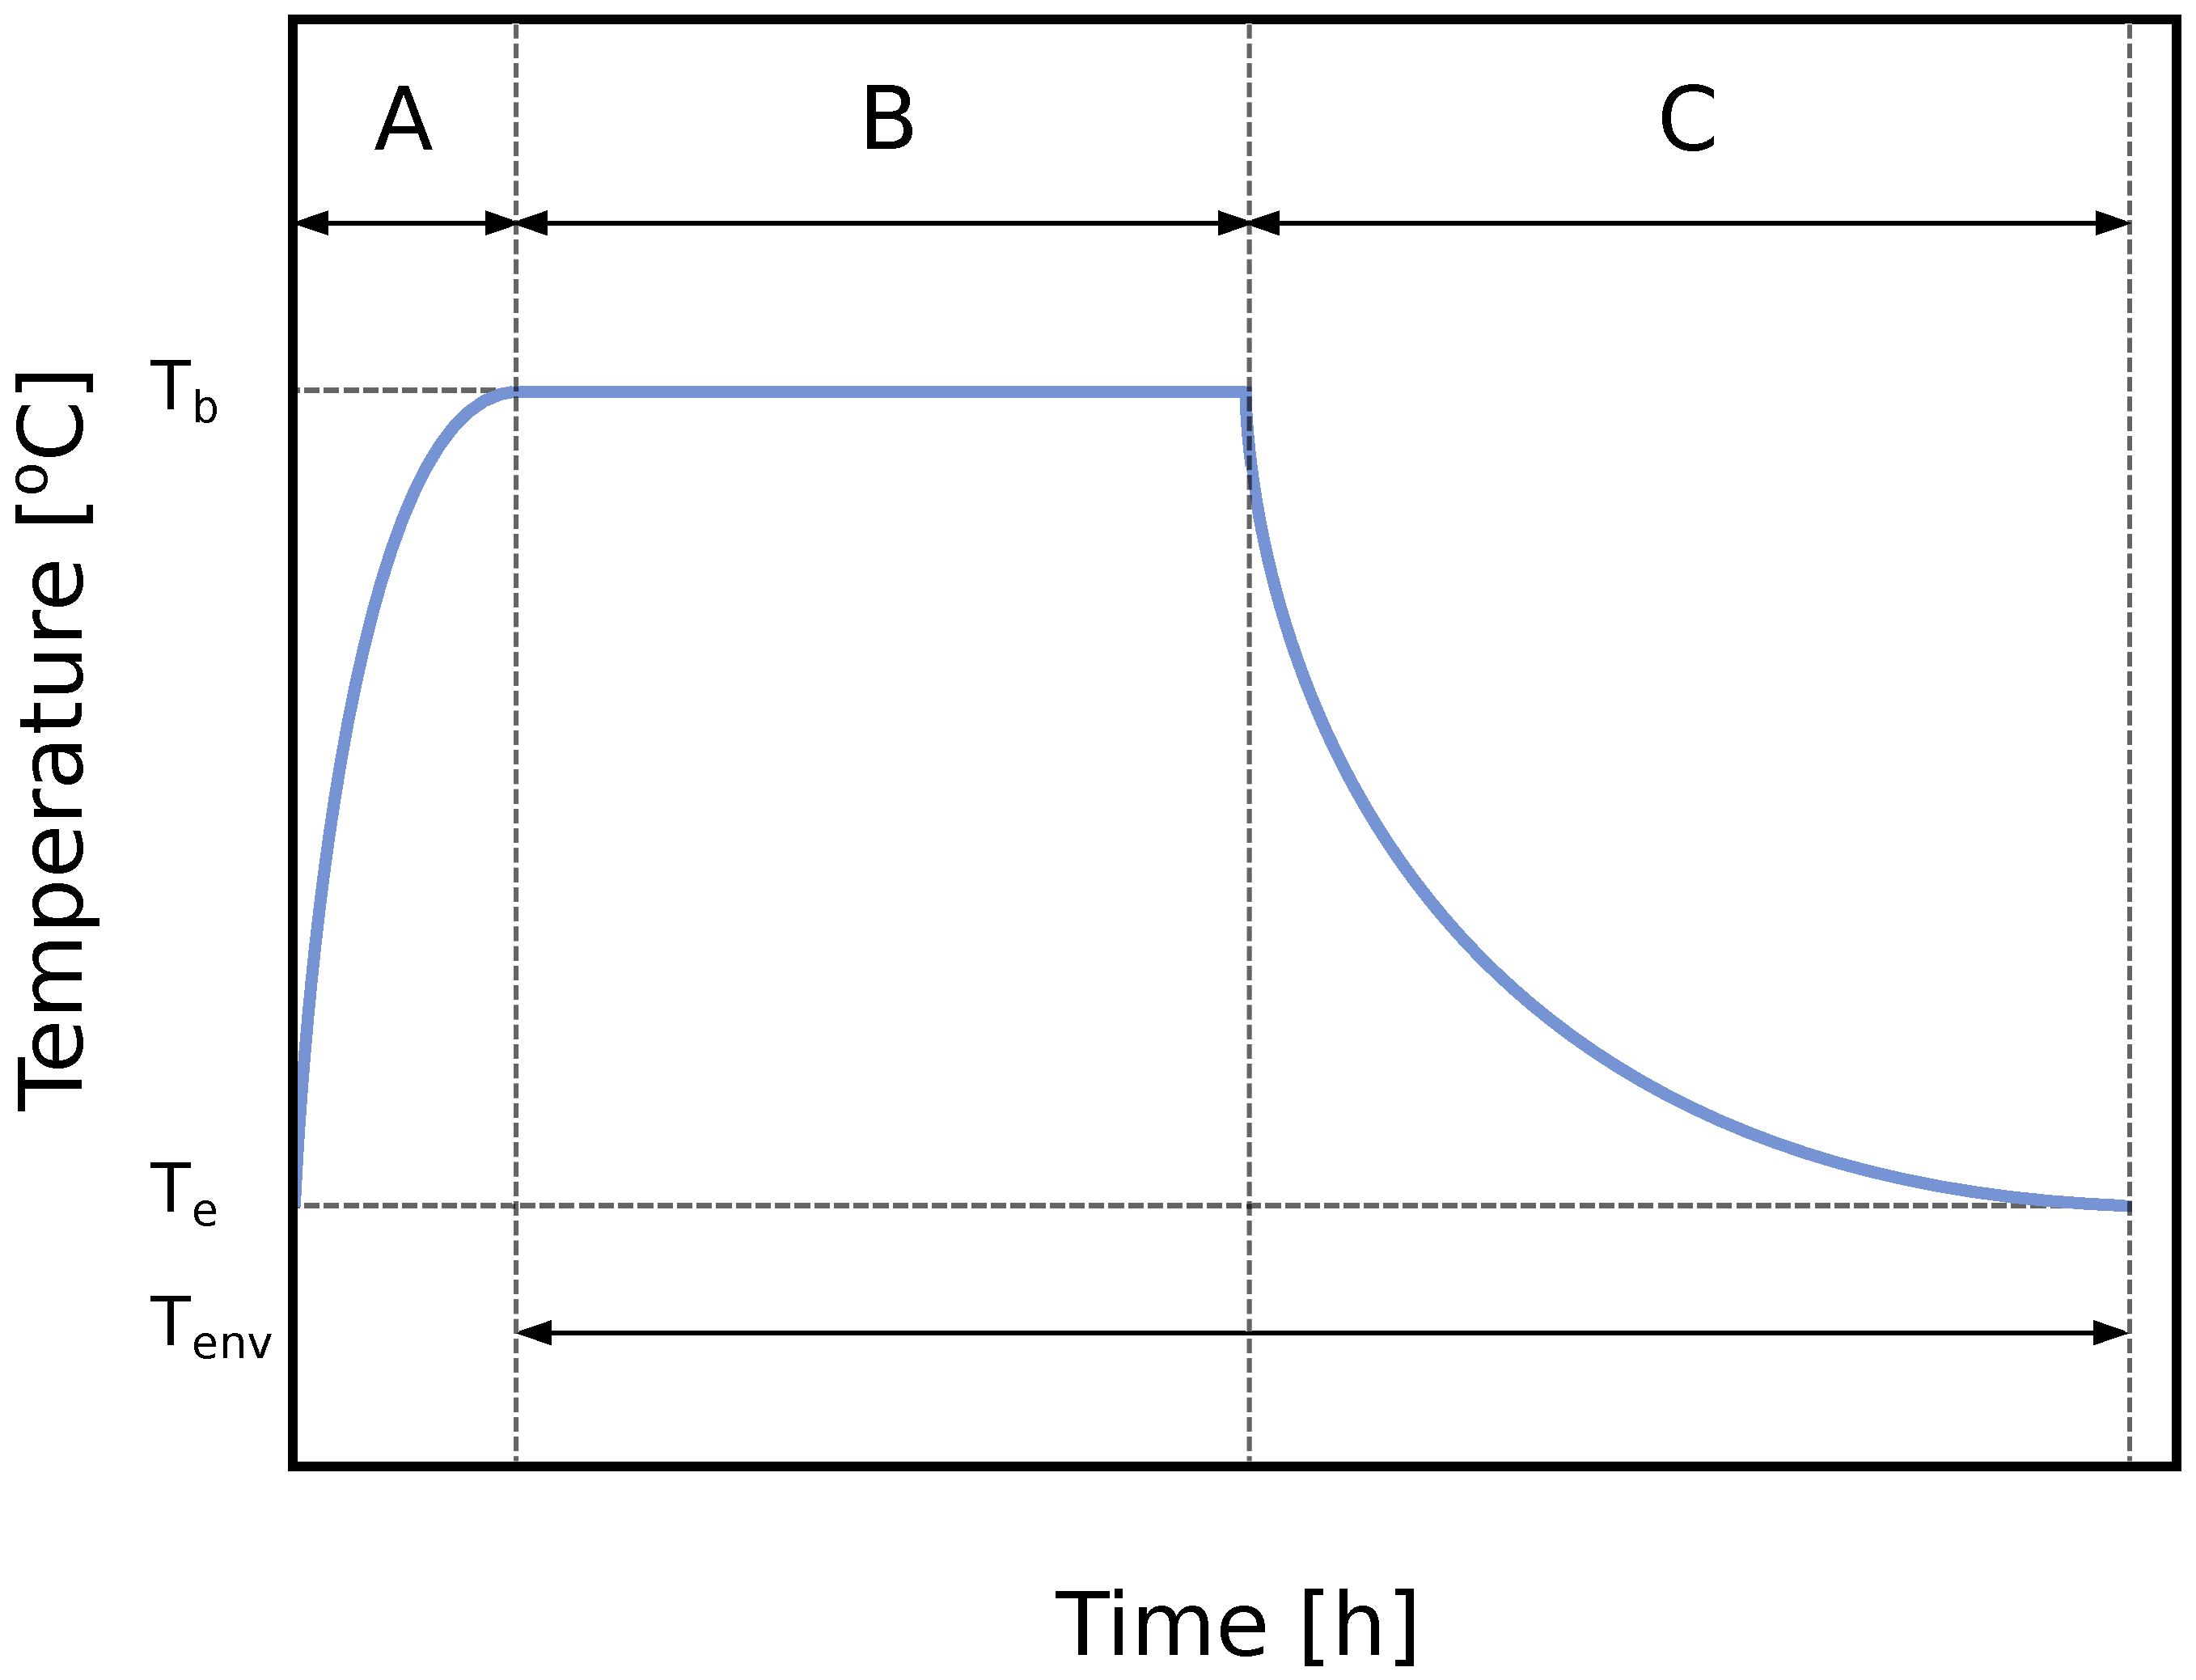
\includegraphics[width=0.63\textwidth]{Pictures/SLS_temp_over_time.eps}\\
        \caption{Phases of an \textit{SLS} process \autocites{Inkscape}{Padovano_SLS_Review}} 
        \label{fig:SLS_temp_over_time}
    \end{figure}

    As seen in figure (\ref{fig:SLS_temp_over_time}), the first phase is the time required to reach a specific powder bed temperature $(T_b)$, based on the material of choice. 

    Ideally this temperature should be maintained constant inside the printing
    chamber, during the entire building phase, through infrared or electric heaters. 
    
    The main goal is avoiding drastic temperature gradients in different areas of the printed part, since they can cause 
    visual artefacts such as local or global deformation and, most importantly, uneven residual mechanical tension that can 
    rapidly degrade the structural integrity of the final piece, especially in structural components that might be placed under static or
    dynamic loads. \\ 
    
    Once the final piece is printed, the entire chamber is cooled down homogeneously and gradually, until the equilibrium is reached at room 
    temperature $(T_e)$ \autocite*{Padovano_SLS_Review}. \\ 

    Quality standards for \textit{SLS} printed parts have increased dramatically over the last few years, to the point where 
    the manufactured components are not exclusively used for prototyping or as sacrificial items for investment casting, but they are 
    used as finalized industrial grade parts. 

    However, there is still room for substantial improvements in the consistency of print accuracy, overall quality, reliability 
    and scalability of the entire process, compared to more traditional manufacturing techniques. \\ 

    The variety of physical phenomena involved in SLS, the fact that they can be interdepent and their different temporal regimes are the main 
    source of complexity that makes the process inconsistent and very hard to study. 

    The most predominant phenomena are the following \autocite*{Padovano_SLS_Review}: 

    \begin{itemize}
        \item Laser motion and irradiation
        \item Thermal diffusion
        \item Polymer viscous flow and particle coalescence 
        \item Powder spreading
        \item Solidification/crystallization 
    \end{itemize} 
    
    Further improvements are required in order to reduce the amount of discarded parts (still comparatively 
    higher than most consolidated manufacturing techniques), usually defective in terms of porosity or 
    thermal distortion or warping \autocite*{Padovano_SLS_Review}. \\ 

    The next chapters will focus on potential SLS materials for this case study and their powder production specifically. \clearpage

    \section{PHAs (Polyhydroxyalkanoates)  \label{PHA_in_general}}

    \textit{PHA}s are a family of thermoplastic polyesters, obtained by hydroxyalkanoic acids via bacterial fermentation, under 
    nutrient depletion and carbon excess conditions \autocites{Kovalcik_PHA_Review}{Messori_Bondioli_PHAs}. 

    They are a sustainable alternative to petrochemical polymers commonly utilized in 
    additive manufacturing and they are mostly used for prototyping in the medical field \autocites{Kovalcik_PHA_Review}{Messori_Bondioli_PHAs}. 

    Similarly to other sustainable plastics, \textit{PHA} can be produced using industrial byproducts as substrates (corn, soy, coffee, oil wastes, etc.)
    \autocite{Kovalcik_PHA_Review}. \\ 

    The monomer composition of PHA can be very diverse, depending on the microorganisms involved and the fermentation medium. 
    
    This variety impacts the overall mechanical, thermal and chemical properties of the final plastic, which depend on the concentration of 
    different monomers in polymers and copolymers. 

    PHAs can be classified by the chain-length of their monomers \autocite*{Messori_Bondioli_PHAs}: 

    \begin{itemize}
        \item \textit{scl-PHA} (short-chain-length PHA) with 3 to 5 carbon atoms
        \item \textit{mcl-PHA} (medium-chain-length PHA) with 6 to 14 carbon atoms
        \item \textit{lcl-PHA} (long-chain-length PHA) with more than 14 carbon atoms
    \end{itemize}


    Estimating the exact meaningful measures of their properties is not always a straight-forward process, 
    since manufacturers are not transparent about the exact composition of their products, which may have been 
    improved by proprietary additives, whose concentration and exact composition are not usually fully disclosed \autocite{Kovalcik_PHA_Review}. \\ 
    
    The market for bioderived PHA has gradually increased over the years and the growth is estimated to keep its pace, given that not only are they more sustainable
    than competing petrochemical polymers, but they offer additional valuable properties, such as piezolectricity 
    and protection against gases and UV lights \autocite{Kovalcik_PHA_Review}.

    Their bio-origin, non-toxicity, renewability, biodegradability and biocompatibility make PHAs a very compelling product in the 
    ever growing market of sustainable materials. 

    However, these desirable qualities contribute to their higher price, which is still not competetive against more established 
    polymers of similar properties \autocite{Kovalcik_PHA_Review}. 

    The increasing demand and the improvements on their biosynthesis will make their price more accessible in the future, for all sorts of 
    applications, including additive manufacturing, where PHAs can be printed successfully either with FDM or SLS techniques. \clearpage

    
    \subsection{PHA and Additive Manufacturing \label{PHA_in_Additive}}

    PHAs can be used in different AM techniques, including Stereolitography, which is part of VP processes (\ref{AM_techniques_summary}), 
    Fused Deposition Modeling (\ref{FDM_general}), where the filaments are made of a mixture of PHA and PLA, 
    (which increases thermal stability and cuts down cost), and 
    Selective Laser Sintering (\ref{SLS_general}) \autocite{Kovalcik_PHA_Review}. \\ 

    This case study will focus on its usage in SLS. \\ 

    PHAs have been successfully printed via SLS and utilized in the medical field as scaffolds for tissues engineering applications. 

    These scaffolds can be printed with a porous structure (controlled by the laser energy density), 
    which could aid in carrying biomolecules and slowly release drugs, for instance.
    
    Unlike with FDM applications, where PHA can not be used as a standalone filament, but needs PLA addition in order to stabilize its melting 
    phase, PHA powders for SLS tend to maintain a better stability and their chemical composition does not get altered as easily. 

    This is a clear advantage, since general properties of the final products do not change drastically from its starting feedstock, 
    and, in addition to this, the remaining powder is not thermally altered in proximity to the melt pool, meaning that it can 
    be reused for additional printing \autocite{Kovalcik_PHA_Review}.  \\
        
    \subsubsection{PHBH \label{PHBH}}

    Poly(3-hydroxybutirate-\textit{co}-3-hydroxyhexanoate) is a copolymer of the PHA family, which gained 
    interest in the AM field and specifically in SLS applications, since it has a wider sintering window (\ref{Powder_requirements}) than other polyhydroxyalkanoates
    such as PHB and PHBV \autocites{DechetMaximilianA2020OtDo}{doi:10.1063/1.4918516}. \\ 
    
    Despite having gained attention in the PHA family for SLS, especially in academic environments, the general interest for this copolymer
    is still relatively lower than other 
    petrochemical polymers, due to its early-stage synthesis process, its cost and the strict confidentiality 
    of polymer manufacturers \autocite{Eraslan_PHBH_review}.  \clearpage

    \section{PBS (Polybutylene Succinate) \label{PBS_in_general}}

    PBS is an eco-friendly biopolymer, which rose interest among 
    industrial and academic environments. It possesses excellent properties and major benefits over comparable materials, as well as some minor drawbacks, 
    which currently hold back its full potential. \\ 
    
    While generally brittle, relatively expensive and still challenging to manufacture in SLS-ready powders without compromises on its environmenal 
    impact (see \ref{Environmental_impact}), this polymer has very desirable features, such as high processability 
    (with traditional methods, at least), flexibility, as well as visual clarity and specularity. 

    It is also thermally stable and its melting point is around $115 \ \celsius $, which can make its processing, generally speaking, 
    less energy wasting, especially when mass production is taken into account. 

    PBS is also easy to blend with other materials; for instance, 
    its mechanical and thermal properties can be drastically improved when used in composite materials, where long or short fibers (or 
    even particles) can be either randomly distributed, or woven into the polymer matrix.
    
    Not only are fibers used for producing high tech composite materials with improved properties, but cheap natural fibers, such as 
    palm fibers, or even blends with starches, can be utilized as an effective way to cut down cost in 
    conventional applications, i.e. food packaging \autocite{Rafiqah_Khalina_PBS_review}.
    
    


    \clearpage

    \section{PBAT (Polybutylene Adipate Terephtalate) \label{PBAT_in_general}}

    PBAT is one of the most promising biopolymers in the sustainable plastics market, since it is very eco-friendly and, at the same time, 
    more performant than comparable alternatives such as PHAs, which exhibit poor mechanical and thermal properties, whereas PBAT is closer to 
    higher performance petrochemical polymers such as polyethylene terephtalate (PET) and polybutylene terephtalate (PBT) 
    \autocites*{Jian_PBAT_overview}. \\

    Currently used mainly in food packaging and agriculture, similarly to PBS \ref{PBS_in_general}, PBAT can be blended with other materials, either 
    for technical enhancing or cost reduction.  

    The considerations made for PHAs and SLS \ref{PHA_in_Additive} should be applicable to both PBS and PBAT, but further experiments need to 
    be conducted and more reliable data needs to be acquired, although different studies are already showing promising results.  

    \clearpage

    \section{Powder production for SLS \label{Powder_production}}

    Manufacturing raw materials for FDM is a relatively easy process, since the plastics need to be mass produced into filaments or pellets \ref{FDM_general}.

    Producing powders from plastics is a much harder process. \\ 

    Two radically different approaches are possible, each with its own critical issues: 

    \begin{itemize}
        \item Mechanical milling
        \item Chemical precipitation
    \end{itemize} 

    \subsection{Powder requirements for SLS \label{Powder_requirements}}

    The success rate of SLS prints is highly dependent on the characteristics of the powders involved. 

    The key factors in powder quality are particle size distribution, morphology, as well as thermal, flow and optical properties. \\
    
    Ideally, a gaussian distribution, with most particles close to the average size is desirable, 
    with a tipical range of $(20 \div 80) \ \mu m$ \autocite*{doi:10.1063/1.4918516}. 

    The average particle size directly influences the layer thickness in the SLS process.  
    
    Particle morphology is crucial in the sintering mechanism, where regular, smooth and non-hollow spherical 
    geometries are preferrable \autocite*{doi:10.1063/1.4918516}.  

    \begin{figure}[h!]
        \centering
        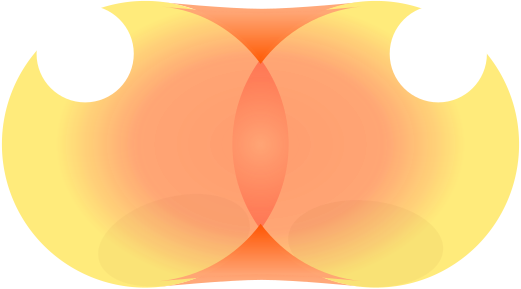
\includegraphics[width=0.5\textwidth]{Pictures/sintering_neck.eps}\\
        \caption{Two spherical powder particles forming a sintering neck \autocite{Inkscape}} 
        \label{fig:SLS_sintering_neck}
    \end{figure}

    The powder's density is another parameter that should be considered, as it directly correlates with the final part's 
    global density and it allows calculation of the Hausner ratio $H_r$, which is a direct predictor of powder flowability. 
    
    Ideally, this coefficient should be lower than 1.4, otherwise the powder could result in issues with fluidization \autocite*{doi:10.1063/1.4918516}. 

    \begin{equation}
        \phantomsection
        \label{eq:Hausner_ratio}
        H_r = \frac{\rho_{tap}}{\rho_{bulk}}
    \end{equation} 

    where $\rho_{tap}$ is the tap density and $\rho_{bulk}$ is the bulk density of the powder. 

    \clearpage



    Understanding thermal properties of the powder is essential in SLS. 


    SLS is characterized by an optimal sintering window, with a temperature range between
    crystallization $(T_c)$ and melting $(T_m)$. 
    For any given heat flow within that range, the material is in a metastable phase, 
    where full coalescence of the top powder layer, as well as adhesion with previously sintered layers are 
    most likely guaranteed \autocite{doi:10.1063/1.4918516}. 

    Therefore, creating a tailor-made powder feedstock involves using materials with a wide enough 
    sintering window \autocites*{DechetMaximilianA2020OtDo}{doi:10.1063/1.4918516}. \\

    Furthermore, optical properties of the powder bed need to be taken into account, since highly reflective materials (for a given 
    laser wavelength) can waste most of the energy input, instead of absorbing a significant amount of radiation needed to 
    effectively melt the powder \autocite{doi:10.1063/1.4918516}.  

    This issue is prevalent in metal SLM \ref{SLS_general}, especially with aluminum. 
    
    However, when it comes to SLS and plastics powders, the required energy is substantially lower than that needed to melt metal alloys, 
    meaning that any potential problem with poor radiation absorbtion can be compensated by increasing the 
    laser power output \autocite{doi:10.1063/1.4918516}. \\ 
    
    Viscosity and surface tension of the melt pool are more relevant factors when choosing powders for SLS. 
    High viscosity and surface tension can hinder the coalescence of polymer powders and the adhesion with previously 
    sintered layers, resulting in residual sheer stress, high porosity and thus poor quality of the 3D printed part in general. 
    
    In SLS, unlike other processes i.e. investment casting or injection molding, there is no well distributed force
    (e.g. built up pressure against the mold) that can increase particle coalescence and layer adhesion. The only relevant
    force acting on the printed part is gravity, along the vertical axis \autocite*{doi:10.1063/1.4918516}. 

    \subsection{Mechanical milling \label{Mechanical_milling}}

    Grinding plastics into fine and homogeneous powders can be a challenge, since the high speed milling devices can easily overheat the 
    plastics above their softening point, creating lumps of material, far from the desired result.
    
    A solution to this problem is using so called \textit{cryogenic grinding} devices, which utilize cooling agents such as dry ice, liquid 
    carbon dioxide or liquid nitrogen, in order to keep the plastics below the glass transition point, where polymers become intrinsically
    brittle, similarly to a ceramic material, making it possible to turn the original mass into a powder \autocites*{cryogenic_grinding_video}{Junghare_cryogenic_grinding_review}. 

    The heterogeneous powders can later be sieved and separated, based on their different granulometry. \\ 

    Despite being an effective process for powder production, the morphology obtained with cryogenic milling is extremely irregular 
    and unpredictable, which makes this method generally unsuitable for high quality SLS parts \autocite*{doi:10.1063/1.4918516}. 

    \subsection{Chemical precipitation \label{Chemical precipitation}}

    There is little variety in the market of SLS ready polymer powders, with polyamide-12 (PA12) being the most optimized for this 
    application and being produced by precipitation in ethanol \autocite*{DechetMaximilianA2020OtDo}.
    
    Many other polymer powders can be produced using the precipitation method, but their development is currently very limited 
    and in early-stage, especially with thermoplastics, which are not as optimized as PA12.
    
    Most of the experimental work on the precipitation method for thermoplastics is not made available by large chemical corporations, 
    but rather by academic environment. 

    \subsubsection{Polymer-Solvent System \label{polymer_solvent_system}}

    Assuming there is a potential material to use this technique with, the recommended solvent choice gravitates towards 
    so called \textit{moderate solvents}. \\
    
    These compounds have the peculiarity of acting as a solvent only when heated above a certain temperature. 

    Therefore, thermoplastics can be dissolved into a compatible solvent and form a liquid-liquid phase separation
    upon cooling of the system, where complex crystallization and precipitation phenomena are later induced via stirring of 
    the nucleated polymer-rich droplets \autocite*{DechetMaximilianA2020OtDo}.  \\ 

    A common criterion of solvent pre-selection is the evaluation of Hansen parameters, through the following equation: 

    \begin{equation}
        \textit{f} (\delta_x) = 100 \cdot \frac{\delta_x}{\delta_d + \delta_p + \delta_h}
        \phantomsection
        \label{eq:hansen_parameters}
    \end{equation}

    which quantifies the interaction between the polymer and the solvent, in correlation with the dispersion $(\delta_d)$, 
    the polar interactions $(\delta_p)$ and the hydrogen bond interactions $(\delta_h)$ \autocite*{DechetMaximilianA2020OtDo}. 

    Once the polymer-solvent system is tested, the experimental data can be effectively represented in the TEAS plot, which 
    helps visualizing the equation (\ref{eq:hansen_parameters}). 

    \begin{figure}[h!]
        \centering
        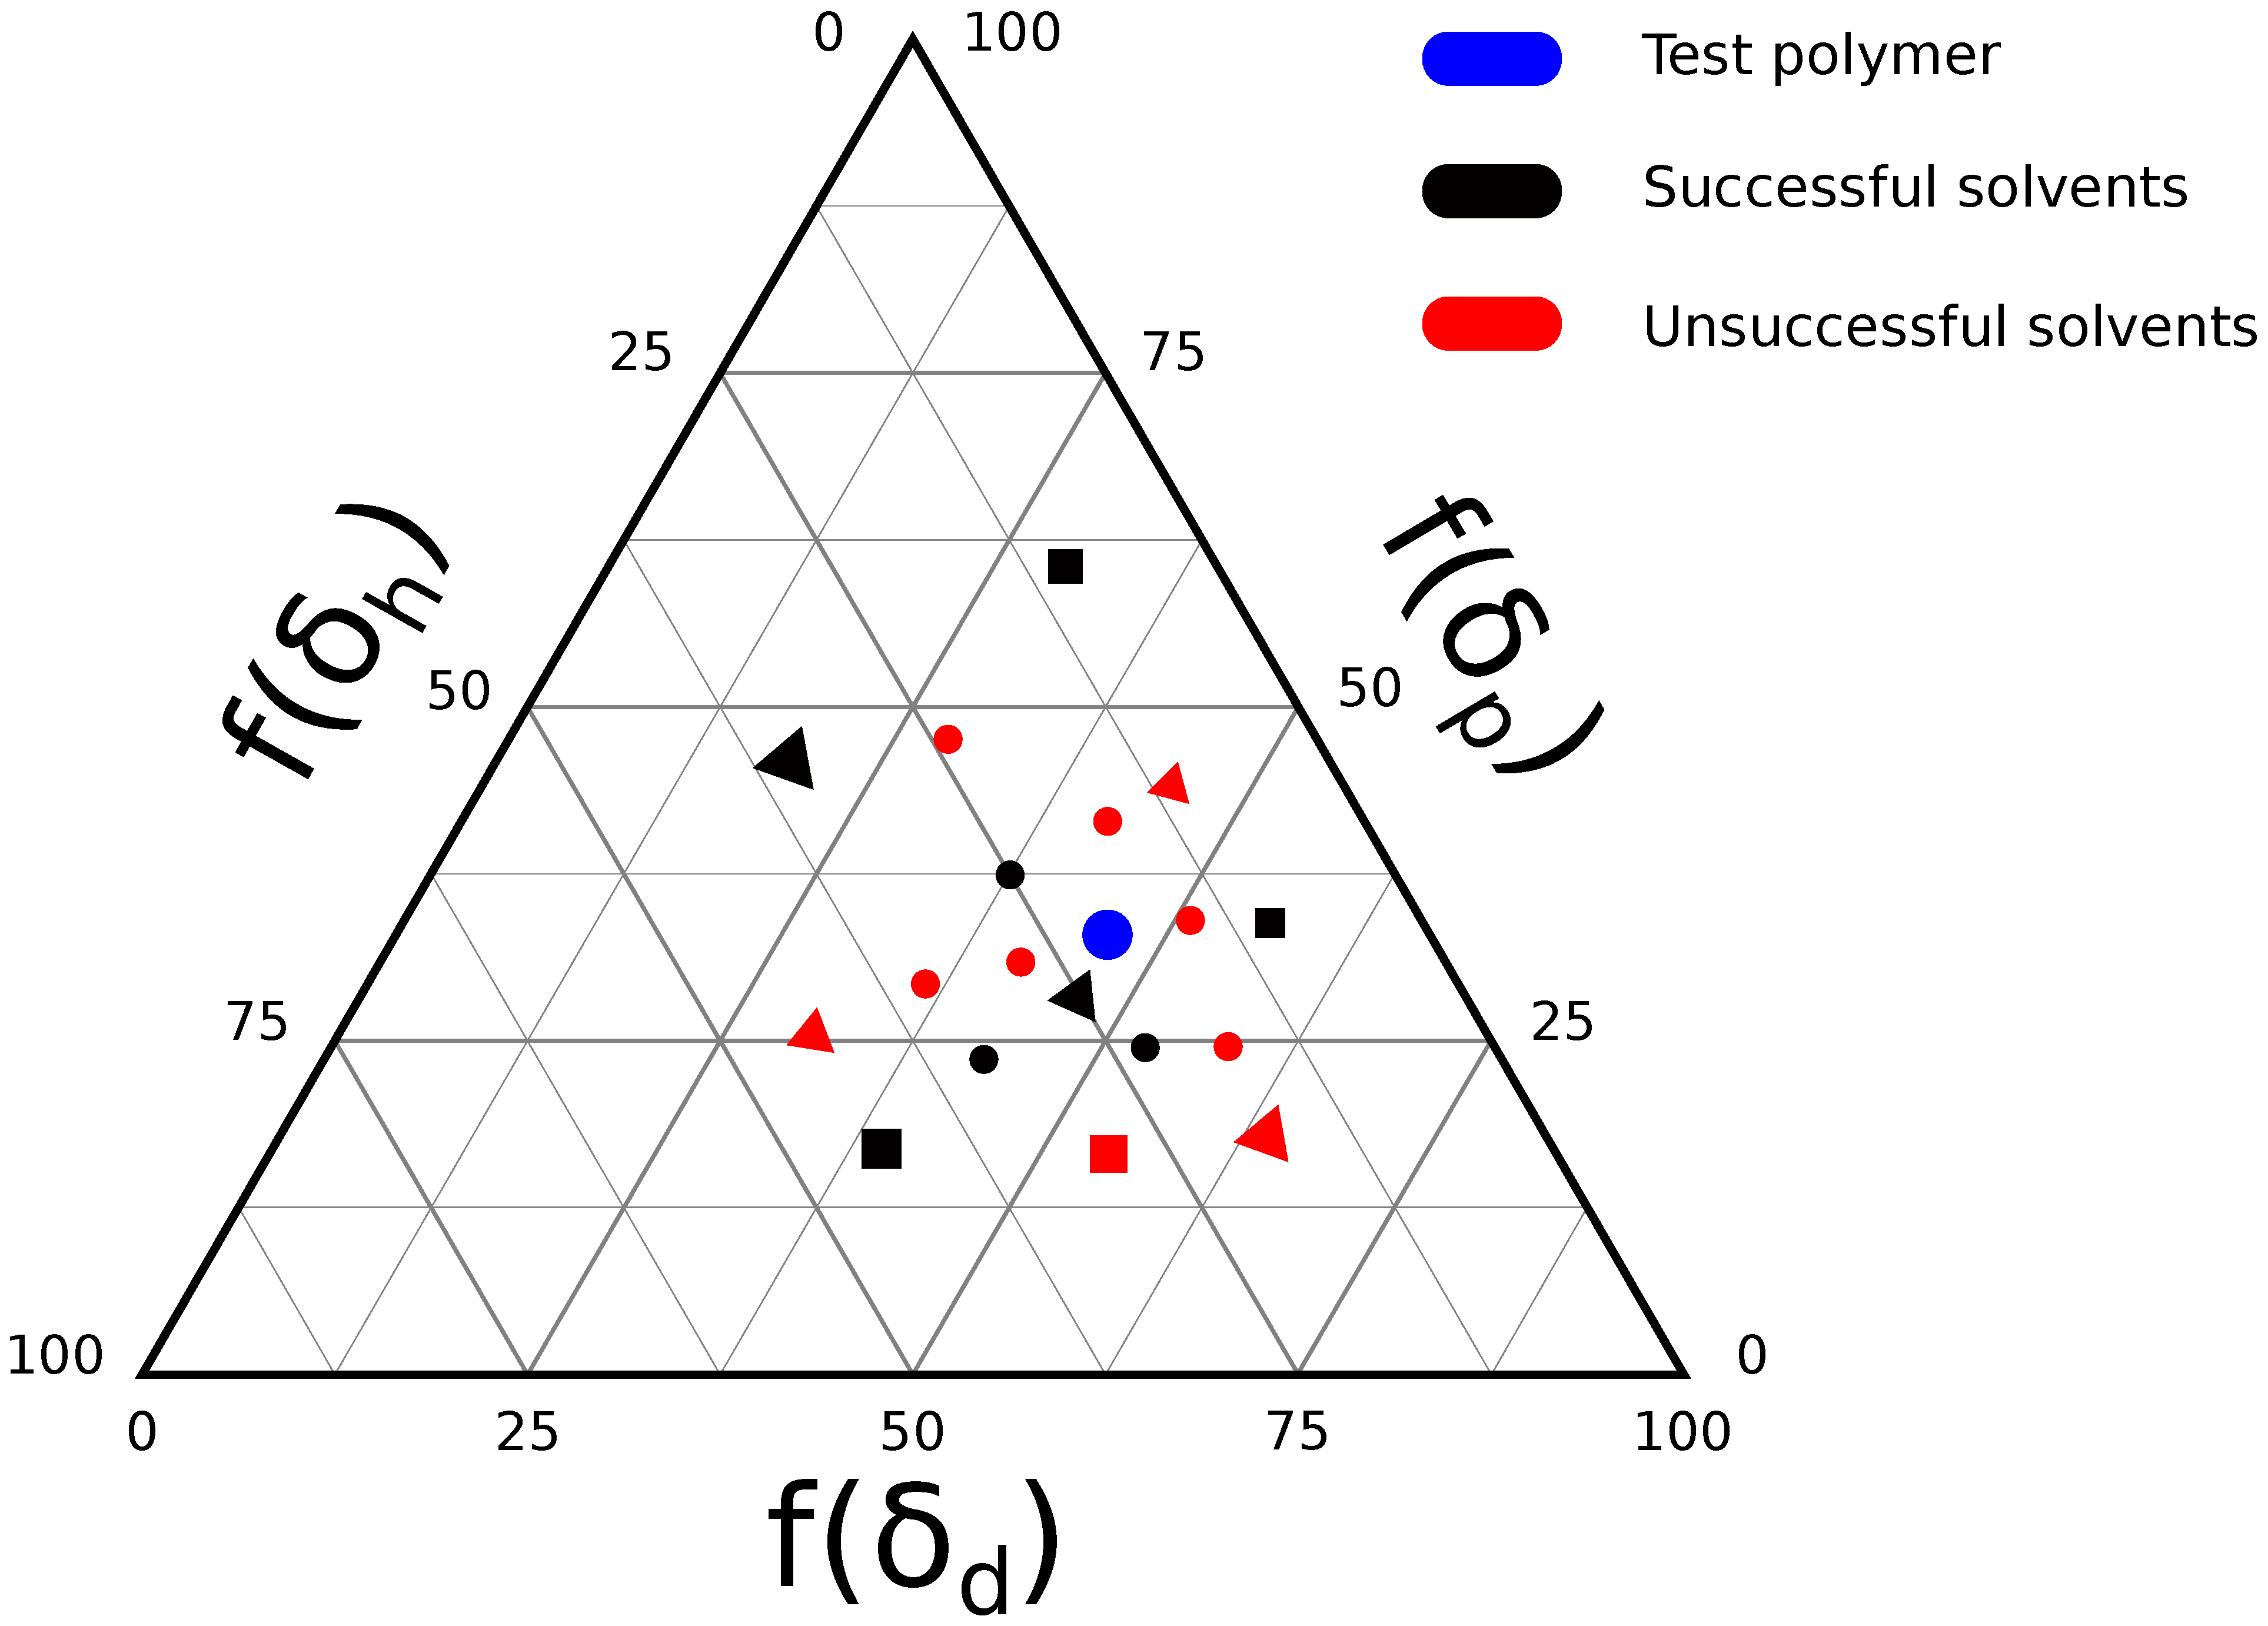
\includegraphics[width=0.4\textwidth]{Pictures/TEAS_plot.eps}
        \caption{Generic TEAS plot for any given polymer \autocites{DechetMaximilianA2020OtDo}{Inkscape}}
        \label{fig:TEAS_plot}
    \end{figure}


    This approach has been successfully used to determine solubility of polypropylene (PP), polyethylene terephtalate (PET), 
    polycarbonate (PC), etc, and could be effectively utilized with the target biopolymers, polybutylene succinate (PBS)
    (\ref{PBS_in_general}), 
    polybutilene adipate terephtalate (PBAT) (\ref{PBAT_in_general}) and with polyhydroxyalkanoates (PHA) such as PHBH (\ref{PHA_in_general}).
    
    

    \subsubsection{Cloud point diagram \label{Cloud_point_diagram}}

    After choosing a suitable moderate solvent, the process needs to be studied and quantified 
    with a cloud point diagram of temperature, as a function of polymer weight concentration, allowing the identification of a dissolution 
    temperature and the temperature where LLPS (liquid-liquid phase separation) occurs. 
    
    These measures allow better scalability of the process in larger controlled environments such as a reactor or autoclave system \autocite{DechetMaximilianA2020OtDo}.
    
    \subsubsection{Production in a controlled environment \label{precipitation_production_controlled_environment}}

    The cloud point diagram data allows for an optimization of the production process in autoclave or reactor system. 

    Temperature profile, initial polymer concentration and, most importantly, stirring conditions can greatly influence the final 
    particle size distribution. 
    
    Stirring is the most impactful of these factors, producing smaller particles as the intensity increases. 

    \begin{figure}[h!]
        \centering
        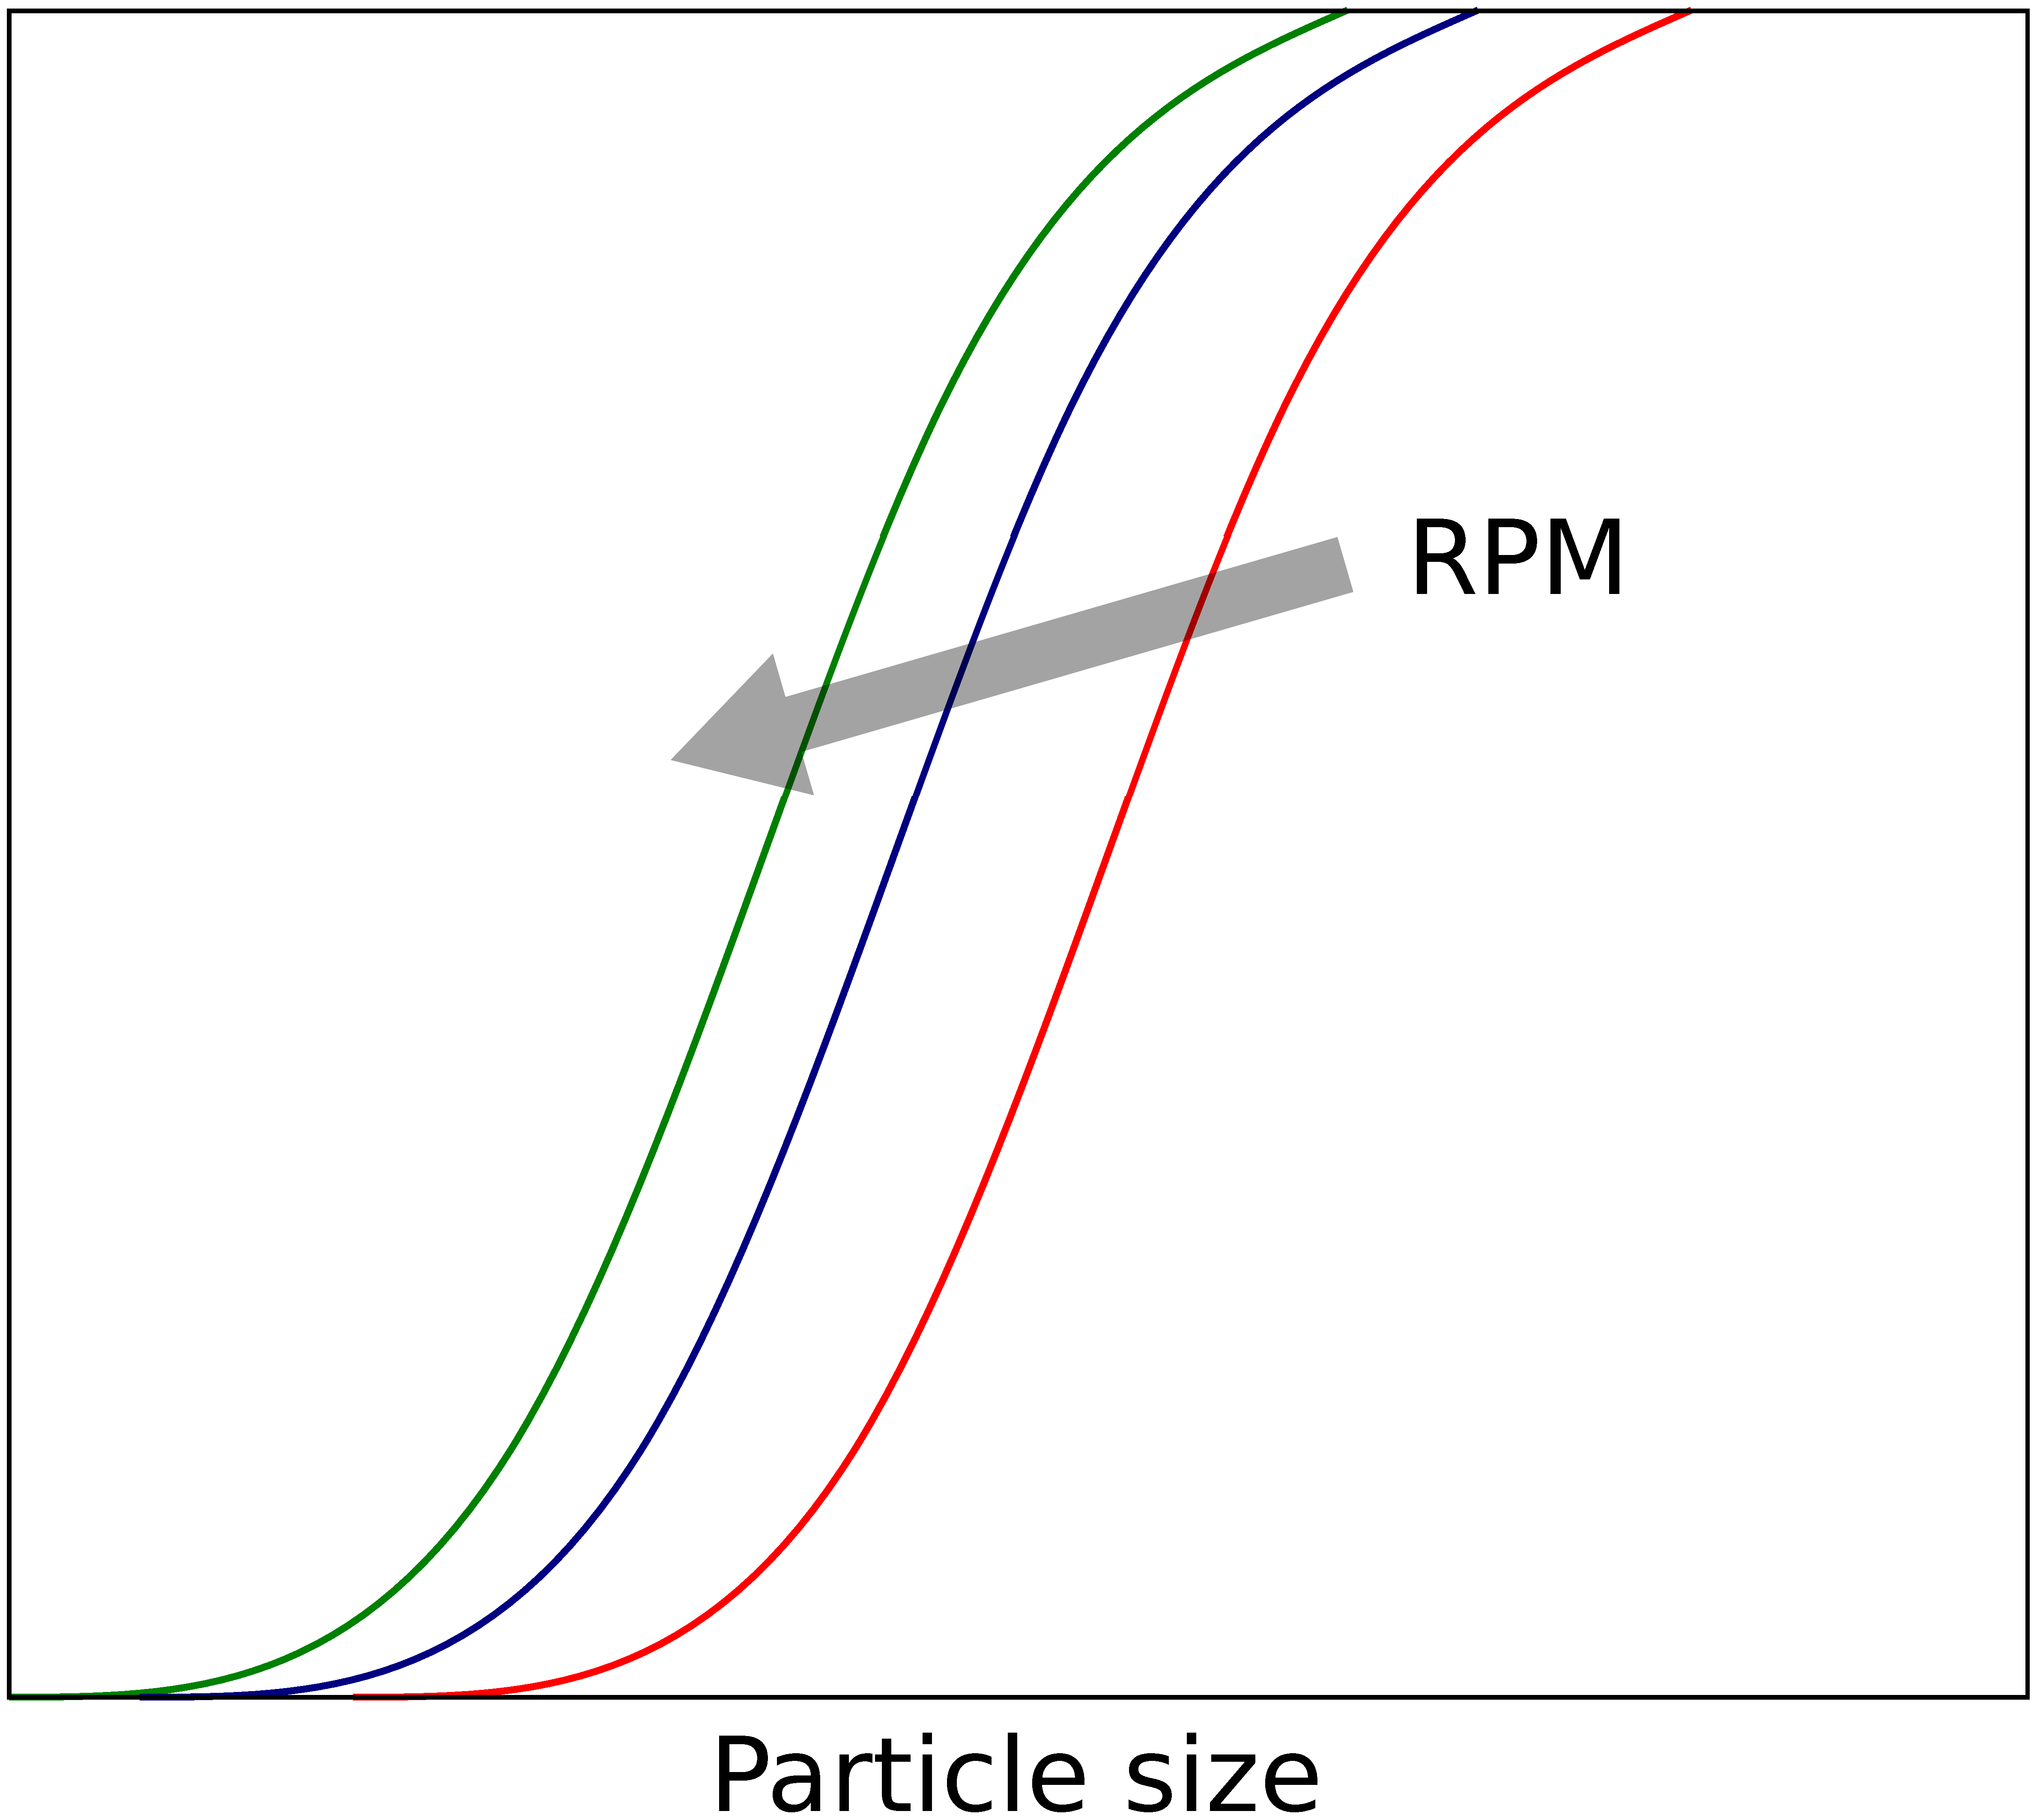
\includegraphics[width=0.5\textwidth]{Pictures/particle_size_stirring.eps}
        \caption{Particle size decreases as stirring RPM increase \autocites{DechetMaximilianA2020OtDo}{Inkscape}}
        \label{fig:stirring_rpm}
    \end{figure}

    \subsection{Environmental impact \label{Environmental_impact}}

    At first glance, cryogenic milling seems to be a more sustainable option for powder production. However, the issues discussed in \ref{Mechanical_milling}, 
    make this method unsuitable for SLS, unless future development will improve overall powder morphology, perhaps with the aid of 
    post processing via thermal rounding of the particles \autocite{DechetMaximilianA2020OtDo}. \\ 
    
    On the other hand, while powder production by 
    chemical precipitation produces much better and more 
    controllable powder feedstock, it is worth noting that organic solvents are intrinsically environmentally impactful and that should be taken 
    into account, especially for large scale production of these powders. 

    The entire purpose of utilizing sustainable biopolymers in the first place might be rendered pointless, if their powder production 
    utilizes compounds or processes that are not environmentally friendly. \\ 

    Better innovative solutions (or mitigations of the mentioned issues in the current pipelines) need to be implemented in the near future. \\ 

    Thermal rounding is a heat treatment, aimed at improving the bulk powder morphology for SLS applications. 
    This kind of treatment might be the crucial step in the success of a more environmentally friendly pipeline, which does not involve 
    any polluting solvent.

    Powders can be heated either directly, with a carrier gas, or indirectly, using heated walls. 

    While the former method has a better process yield and reduced risk of lumping, the latter produces powders with 
    a better, more spherical morphology, but with a significantly higher risk of particle agglomeration \autocite{Dechet_Schmidt_thermal_rounding}.

    \clearpage

    \section{Laboratory environmental conditions and available equipment\label{Lab_condition_equipment}}

    The experimental phase of this case study has been conducted in various laboratories at \textit{DISAT@PoliTo}. \\ 

    The main production process (\ref{Choice_material_process}) has been studied and optimized in 
    the \textit{Tape Casting} lab, then the residual moisture of each - cleaned and 
    unsieved - batch of powder has been removed in an oven at the \textit{Burner Rig} lab (\ref{Choice_material_process}).

    Several powder samples, collected at different phases of the optimization process, have been analyzed 
    with a \textit{SEM} (Scanning Electron Microscope) at a third party 
    facility (\ref{SEM_analysis}), and subjected to 
    a \textit{TGA} (\ref{TGA_Analysis}) and a \textit{DSC} (\ref{DSC_analysis}) 
    at the \textit{Thermal Analysis} lab of the same department. \\ 
    
        \subsection{Tape Casting lab\label{Tape_casting}}

        The laboratory has a large workbench and is stocked with all sorts of useful tools and equipment, especially flasks,
        beakers and glassware 
        in general, as well as a chemical hood, which was essential for a safe use of chloroform 
        (\ref{Initial_recipe}, \ref{detailed_reaction}). \\ 

        A huge problem of this specific laboratory were the uncontrolled environmental conditions. \\

        The extremely high summer temperatures (usually close to $40 \ ^{\circ} C$ and never lower than 
        $30 \ ^{\circ} C$) drastically accelerated the evaporation of chloroform, which resulted in a 
        very viscous PHBH solution that either ended up in a very low yield, or entirely disrupted the 
        precipitation process by clogging the drippers (\ref{Initial_recipe}, \ref{recipe_improvement}).

        The uncontrolled humidity was another factor that hindered the production pipeline, given that the very 
        fine powders are extremely hygroscopic and prone to creating hard to separate lumps. \\ 
        
        These critical issues led to several adaptations and better choices among the available pieces of
        equipment (\ref{recipe_improvement}, \ref{faulty_equipment}), as well as tweaking of the precipitation 
        reaction, which in turn increased the pellet-to-powder yield by over ten-fold, compared to the initial 
        results (\ref{initial_failures}).



    \clearpage
    \section{Choice of material and production process\label{Choice_material_process}}

    As seen in previous chapters, samples of PHBH (\ref{PHBH}), PBAT (\ref{PBAT_in_general}) and 
    PBS (\ref{PBS_in_general}) were available for this experimental phase. \\ 

    An early stage precipitation reaction had already been developed for PHBH, by other researchers at \textit{Disat@PoliTo}. 
    This initial recipe (\ref{Initial_recipe}) has been tested out with the other biopolymers as well, but PHBH held the most promising 
    results even in its early stages. \\ 

    Other approaches such as cryogenic milling (\ref{Mechanical_milling}) have been briefly tried, but quickly 
    discarded, due to the lack of equipment suitable for thermal rounding treatments. 

    The grinding procedure, aided by liquid nitrogen, proved to be successful at producing fine powders. 

    However, unless a thermal rounding treatment is applied, the powder 
    morphology is too irregular and far from the ideal spherical geometry, thus making the 
    obtained batches unsuitable for 3D printing. \\  

    All of the mentioned points led to choosing PHBH for this case study, focusing on the optimization of 
    the available blueprint for a suitable chemical 
    precipitation process (\ref{Initial_recipe}, \ref{detailed_reaction}, \ref{recipe_improvement}). 

    \clearpage
    \section{Initial chemical precipitation recipe for PHBH\label{Initial_recipe}}
    
    Researchers at \textit{DISAT@PoliTo} started developing a prototype for a chemical precipitation reaction, 
    derived from experiments on solute-solvent compatibility (\ref{fig:TEAS_plot}), 
    which highlighted a good affinity between PHBH and chloroform. \\ 

    Starting from a 4 g batch of PHBH pellets, the highest amount of sieved powder ($ < \ 100 \ \mu m$ )
    ever produced was around 1.2 g, resulting in a $30 \ \% $ maximum yield. \\ 

    The very early experiments were conducted in the \textit{Tape Casting} Lab, with the issues previously discussed 
    (\ref{Tape_casting}) playing a major role in the reaction's rate of success. 
    
    The environmental conditions at the time were drastically different compared to those experienced during the latest experimental 
    activities. 

    Most importantly, the lab temperature was substantially lower, as the reaction was prototyped during winter. 
    
    As earlier mentioned (\ref{Tape_casting}), the extremely high summer temperatures dramatically increased the evaporation rate of 
    chloroform, leaving a high viscosity solution that was harder to control during precipitation. \\

    This led to failures and practically insignificant yields (\ref{initial_failures}) if 
    the reaction succeeded, when testing the recipe in these conditions.  

    After thoroughly studying the process in all its phases and isolating different variables that could have caused the issues, 
    the recipe has been tweaked and adapted to the external conditions, which is later discussed 
    in detail (\ref{recipe_improvement}, \ref{key_variables}). 

        \subsection{Components\label{Components}}

        The ingredients and quantities of the prototype reaction were the following: 

            \begin{itemize}
                \item 4 g of PHBH pellets 
                \item 55 ml of chloroform 
                \item 400 ml of $0.25 \ \% $ (by weight) of PVA solution 
            \end{itemize}

        Despite its simplicity, the reaction is highly influenced by the environmental conditions, as well as
        equipment's correct use and proper operability. \\ 
        
        Any slight deviation from the correct parameters, whether due to 
        unpredictable changes in environmental conditions, malfunctioning or incorrect use of the available tools, could 
        in fact potentially break the unstable equilibrium of the reaction, making it extremely 
        hard to pinpoint the exact root cause of failure. \\  

        Several failed attempts, changes in equipment and tools, as well as quantities were required in order 
        to understand the most relevant parameters of the entire process. 
        \subsection{Equipment\label{Equipment}}

        All the essential pieces of equipment and tools for the reaction are listed here: 

            \begin{itemize}
                \item Clean flasks and glassware for volumetric measurements, waste containment and disposal, etc
                \item A high precision weight scale 
                \item A magnetic stirrer and heater 
                \item Appropriately sized stir bars \footnotemark 
                    \footnotetext{An inadequate stir bar size, in comparison to the stirring container, can 
                    be unstable and stop stirring or create undesired foams and splashes}
                \item Appropriately sized beakers for the PHBH-chloroform and the PVA solution \footnotemark 
                    \footnotetext{An adequately sized and shaped container is required for the same reason}
                \item A flow controllable dripper 
                \item A chemical hood \footnotemark
                    \footnotetext{A chemical hood is generally required to safely operate with chemicals that produce 
                    vapours or fumes. Chloroform evaporates extremely quickly and is mildly toxic. Suddenly inhaling 
                    a large amount can cause a human to lose consciousness}
                \item Distilled water for powder and tool cleaning 
                \item A vacuum ejector 
                \item A fritted glass filter or a paper filter \footnotemark
                    \footnotetext{A porous filter combined with a vacuum ejector is preferred, as it 
                    exponentially decreases powder filtering and cleaning time} 
                \item An oven or dehydrator
                \item A sieve \footnotemark
                    \footnotetext{A ($ < \ 100 \ \mu m$ ) sieve was available, but smaller 
                    sizes ($20\div 80 \ \mu m$) could be required}
                \item Sealed test tubes or any other container suitable for fine powders storage \footnotemark
                    \footnotetext{Electrostatic attraction to different materials can cause significant powder losses over time}
            \end{itemize}



        \subsection{Detailed step-by-step reaction\label{detailed_reaction}}

        The reaction is shortly described by the following diagram: \\ 

        PHBH pellets (4 g) need to be dissolved into 55 ml of chloroform, in order to create a viscous liquid that will later be slowly dripped into a 
        $0.25 \ \%$ PVA solution, where the precipitation occurs for a duration of 7.5 hours, at 700 rpms. \\ 

        Depending on the recipient used to contain the viscous solution, the stir bar should be appropriately sized and 
        the stirring speed should be adjusted accordingly, in order to minimize evaporation and avoid the formation of foams and 
        splashes of chloroform. \\ 
        
        Way too low speeds will in fact result in a long stirring time and excessive evaporation of chloroform, which leads to 
        higher viscosity and issues with the formation of fine powders during precipitation, as previously discussed (\ref{Tape_casting}). \\ 

        On the other hand, splashes and foaming can occur at excessively high stirring speeds, causing loss of liquid, or
        hindering the visual inspection of the solution, respectively. 

        A visual inspection of the solution is essential, as the presence of undissolved PHBH granules or impurities can 
        obstruct the dripper or potentially drastically reduce the final yield. 

        Chloroform tends to dissolve PHBH's surface extremely quickly, creating a film around each granule, that could potentially stick 
        them together or to the container, which can lead to a significant delay in total dissolution time. 

        It is best practice to slowly drop PHBH pellets into cloroform while already being stirred, instead of pouring 
        the solvent onto the granules, in order to avoid the aforementioned issues. \\ 

        Once the solution is ready, it can be poured into the flow controlled dripper. 

        The flow rate can be controlled through a manual valve and should be adjusted periodically, as the column of fluid diminishes 
        in height with time, reducing the total weight that pushes more fluid down the thin channel. 

        The solution can dry and create a plastic film all around the dripper's walls, reducing the cross section of the last thin 
        trait over time. Flow rate should be manually adjusted to compensate this issue as well. \\ 

        Ideally, the chloroform solution should flow in a fast paced but drop-by-drop fashion. 

        The flux valve can be extremely sensitive and hard to control manually, so occasional large bursts of fluid can suddenly 
        end up in the PVA solution. 

        However, as long as this phenomenon does not occur too frequently and is dealt with in a timely manner by closing the valve and slowly 
        readjusting the flow, it does not seem to affect the precipitation process in a significant way (\ref{key_variables}). \\ 

        The 400 ml of $0.25 \ \%$ PVA solution should be ready in advance and already set at the proper stirring speed, before 
        the dripping process begins. \\ 

        The percentage of PVA is extremely low and it is best practice to prepare a higher concentration solution, in large batches,  
        that can be further diluted and utilized when needed. \\

        Batches of 1 kg PVA solution ($1 \ \%$ by weight) were prepared and stored in a refrigerator. 

        The initial approach was utilizing mass units only, however PVA can be hard to dissolve in water at room temperature. 
        
        Different batches were prepared by gradually increasing the operational temperature, regulated by a magnetic stirrer-heater. 

        Unless water temperature was kept substantially high (above $70 \ ^{\circ}C $ but still lower than boiling point), 
        solid PVA flakes remained undissolved, despite being stirred for hours. 

        Regardless, defective batches were used during the early experiments, but the undissolved PVA 
        seemed to create a slimy solution that, over time, would produce a thick foam, that potentially clogged 
        the fritted glass filters. 

        Temperatures have been kept higher since then, resulting in no filtering issues down the pipeline. \\ 

        However, despite being able to fully dissolve the solute, water evaporated consistently, making it necessary to refill the 
        container with distilled water, until 1 l of total solution was reached. 

        This was clearly an approximation, compared to the initial choice of utilizing mass measurements only, however 
        the error of a volume filling approach can be considered negligible, given that the 
        percentage of PVA is only $1 \ \%$ by weight and the solution needs to be further diluted down to $0.25 \ \%$ for 
        the precipitation reaction. \\ 

        Dilution to the required fraction of mass is simply obtained by using 100 ml of $1 \ \%$ solution, 
        plus 300 ml of water, for a total of 400 ml. \\ 

        The precipitation reaction is left stirring for 7.5 hours under a 
        chemical hood, starting from the very first drop of PHBH-chloroform solution. 

        This time frame is extremely conservative, as it is very likely that all the residual chloroform is entirely 
        evaporated in a much shorter time, however this aspect has not been tested yet. \\

        At the end of the waiting time, the solution can be filtered with a fritted glass filter, aided by a vacuum 
        ejector. 

        After the PVA solution is filtered out, the remaining powder bed should be washed with isopropyl alcohol and 
        distilled water. 

        Paper filters can be utilized, but the filtering phase would last exponentially longer. Furthermore, the vacuum filtering 
        approach can get rid of almost all of the residual moisture. \\ 

        The obtained powder bed needs to be dried in an oven or a dehydrator, at $40 \ ^{\circ}C$, for at least 12 hours. \\ 

        At this point, the powder should be completely dry and ready to be sieved. \\ 

        A $100 \ \mu m$ sieve has been used, however, smaller size sieves could be used, as many reviews recommend a particle 
        size of $20 \div 80 \ \mu m$ for SLS \ref{SLS_general}. 
        
        Powders should be gently pushed against the mesh, alternating with circular motion and shaking of the sieve, should 
        an automated sieving system be unavailable. 

        Several passages might be needed in order to collect most of the powder. \\ 

        Sieved powders should be immediately stored in test tubes or any other sealable container, as they are extremely hygroscopic. 

        With very fine powders, electrostatic interactions with tools and materials should be taken into account, when transferring 
        them into containers. 

        Some losses are expected during this phase, unless specific tools for collecting very fine powders are available. 

        Choosing appropriate materials and reducing material transfer to the minimum amount is essential to minimize 
        powder losses. 

        All tools and containers should be perfectly dry too. 



        \subsection{Initial results and failures\label{initial_failures}}

        As mentioned in previous chapters (\ref{Tape_casting}), many failed attempts led to a deeper understanding of the entire process 
        and the proper choice of equipment, tools and tweaking of the initial recipe. \\ 

        The most prominent issue were the environmental variables in the \textit{Tape Casting} lab. With temperatures constantly exceeding 
        $30 \ ^{\circ}C$, the 55 ml of chloroform, initially used by previous researchers during winter, evaporated too 
        quickly while PHBH pellets were being dissolved. 

        The obtained liquid was extremely viscous and hard to drip effectively into the PVA solution. Drippers were constantly clogged
        and flow control via manual valves was unpredictable, to say the least. 
        
        A thick plastic film covered the internal walls of the drippers and the beakers where PHBH had been dissolved, which 
        introduced the very first significant material waste point in the pipeline. 

        Moreover, despite being impossible to avoid in general, the excessive thickness of this film that formed in the first batches 
        severely hindered the cleaning and maintenance of the utilized glassware, which occasionally needed to be cleaned with chloroform 
        or other solvents. \\ 

        Despite being able to save most initial batches, the final yield was insignificant, going as low as 0.1 g of powder 
        per 4 g of raw material. \\ 
        
        Another factor that severely reduced production rate was the frequent clogging of fritted glass filters. 
        
        The undissolved PVA flakes in the first defective batches (\ref{detailed_reaction}) created a dense foam, which either obstructed 
        the pores of the filter or slowed the filtration time by orders of magnitude. 

        The clogged filters required to be regenerated with chloroform and rinsed with isopropyl alcohol, in order to regain full 
        functionality. 

        In addition to this, some of the filters initially used had already been exploited by other research teams, operating 
        with metal fines and other materials, which might have contributed to some of the impurities and alien particles detected 
        by SEM analysis in the earliest samples (\ref{SEM_analysis}). \\ 




    \clearpage

    \section{Recipe tweaking and improvements\label{recipe_improvement}}

    All of the aforementioned failed attempts (\ref{initial_failures}) led to an optimization process that originally aimed at 
    matching the $30 \ \%$ yield (\ref{Initial_recipe}) obtained by previous researchers (who provided 
    the prototype recipe but worked in different environmental conditions), but later far exceeded the 
    initial expectations, improving upon the available blueprint procedure by a wide margin. 


        \subsection{Key variables\label{key_variables}}

        Dealing with a simple yet unstable process, based on theoretical studies and very rough experimental data, requires a
        long trial and error approach, that should carefully isolate each variable, whether it is intrinsic to the 
        involved physical and chemical reactions, environmental, equipment related, or introduced by human 
        interaction with the process. \\ 

        Generally speaking, once all the independent variables are isolated and understood, only a few are extremely relevant and can 
        radically influence the success rate of the entire process. 

        Should these variables be changed, even unintentionally and by a small amount, the final yield
        could be dramatically cut down. \\ 

        It has been pointed out several times that the external temperature is one of the most 
        (if not the absolute most) influential parameter of the entire process, given the fast evaporation pace of chloroform, 
        or organic solvents in general, should the reaction be re-engineered with a less impactful solvent, like the moderate 
        solvents often mentioned in the scientific literature (\ref{Chemical precipitation}). 

        This variable could not be controlled, as air conditioning was not present in the \textit{Tape Casting} lab 
        (\ref{Tape_casting}). 

        For all the issues discussed in previous chapters, an increase in external temperature correlates with an increase in 
        chloroform use. Starting from the initial 55 ml per 4 g of PHBH pellets, extra chloroform has been added 
        by 2.5 ml increments, until the process stabilized and yield reached a peak that would not benefit from further 
        increase. 

        Assuming that, in any human operated laboratory, temperatures should not exceeed those experienced during this case study,  
        the maximum useful amount of chloroform (per 4 g of PHBH pellets) would be around $65 \div 70 \ ml$. 

        This range consistently produced the highest yield (\ref{promising_results}) and not only did further chloroform use stall the 
        results, but it proved to be detrimental over a certain threshold ($ > \ 75 \ ml$), as insufficient 
        viscosity would prevent an accurate flow control during the dripping phase. \\ 

        All these adjustments in chloroform quantity are only a consequence of uncontrolled operational temperatures. A 10 ml 
        increase in chloroform use might seem insignificant at a lab scale, but this would translate to significant waste, 
        should the process be scaled to an industrial level (\ref{consistent_reproducibility}). 

        This consideration ties with the environmental sustainability issue (\ref{Environmental_impact}), since organic solvents are 
        inherently impactful and unnecessary waste should not be promoted, especially when sustainable biopolymers such as PHBH are involved. 

        Overall, the key parameter that actually matters is viscosity: very low temperatures can minimize chloroform evaporation, 
        but directly increase density and thus viscosity; on the other hand, liquids at higher temperatures should be inherently 
        less viscous, but the drastic solvent evaporation dramatically increases viscosity, simply by having more PHBH and less 
        liquid proportionally. \\ 
        
        The process should be tailored to obtain a PHBH-chlofororm solution with the ideal viscosity, that allows a perfect dripping 
        phase, while producing the highest pellet-to-powder yield. 

        However, future experiments should focus on achieving this goal with the lowest amount of chloroform possible, which requires 
        being able to control operational temperature. \\ 

        By contrast, other variables like dripping flow (as previously discussed a drop by drop fashion is ideal but occasional 
        flow distruptions do not seem to have a great influence (\ref{detailed_reaction})), or a very precise measure in 
        PVA concentration are not as important for the success of the precipitation process. 

        With a PVA concentration as low as $0.25 \ \%$ and successful reactions even with defective
        solution batches, it is plausible that the precipitation process could be accomplished by 
        substituting PVA with other alcohols such as isopropanol or ethanol or even by simply using distilled water \footnotemark.
        
            \footnotetext{These substitutions would immensely simplify the production of the precipitation solution for the previously 
            discussed issues of dissolving PVA (\ref{detailed_reaction}), but no experiments have been conducted yet} 

        Assuming the adjustment of viscosity and the optimization of the dripping phase have been dealt with, 
        another relevant parameter is the stirring speed of the PVA solution (\ref{detailed_reaction}). 

        The experiments conducted during this case study confirm what has been found in the scientific literature: 
        an increase in stirring speed directly correlates to a decrease in average powder particle size (\ref{fig:stirring_rpm}). 

        However, this correlation is generally measured in terms of RPM, which is an active control of any magnetic stirrer and 
        a good indication of the average rotational speed of the stirred fluid, assuming that the device is properly functioning
        and every other variable is fixed. 
        
        In fact, the RPM controlled by the machine does correlate with the average angular velocity, but does not indicate 
        an exact speed value. 

        For any fixed fluids, should other factors like container size and shape, stirring rod weight and size change, 
        then the average angular velocity would change as well, despite the stirrer being at a fixed RPM value. 

        Since the production rate had been doubled to 8 g of pellets per batch, the reaction has been split into two 
        4 g batches, for lack of single batch capable equipment. 

        Despite perfectly measuring all the quantities and mirroring equipment use for both batches, the magnetic stirrers'
        reported RPM did not match the uneven velocities (even though the utilized models were exactly the same). 

        This aspect is later discussed in further detail (\ref{faulty_equipment}). \\ 

        Once this issue has been partially solved with some workarounds, increasing RPM has proven to be an effective 
        strategy to increase final yield: powders were effectively produced at the initially planned 700 RPM, however 
        most of the powder batch could not be sieved under $100 \ \mu m$. 

        Higher RPM values produced almost no waste during the sieving phase. 


        \subsection{Adaptation to faulty or unsuitable equipment\label{faulty_equipment}}

        Some of the available equipment was not perfectly suited for the necessary tasks or, sometimes, even broken or malfunctioning. \\ 

        For instance, the drippers used for the precipitation reaction had a manual flux valve, which made flow control unpredictable 
        and hard to regulate. \\ 

        The fritted filters initially used had already been utilized for other production pipelines, transferring some impurities
        to the first samples, which are visible in the SEM images (\ref{SEM_analysis}). This required a new filter to be bought 
        and used solely for producing PHBH powders. \\ 

        A major issue was the malfunctioning of one of the magnetic stirrers, which used to stop stirring unexpectedly, for hours at times, 
        while the reaction was not meant to be supervised. This caused a few batches to be lost, since the prolonged absence of 
        a stirring motion did not allow for the precipitation process to occur. 

        The defective stirrer was replaced. However, despite both the available stirrers being functional, a huge discrepancy 
        in stirring speeds was noticeable, as briefly mentioned in the previous chapter (\ref{key_variables}). 

        In spite of the fact that both solutions were prepared identically and the beakers and stirring rods used 
        were exactly the same, one of the stirrers would visibly show a much lower speed at the same RPM value. 

        As a workaround, a satisfying speed (based on previous results in terms of final yield) was set on the slower stirrer, 
        then the much faster stirrer was set at a "lower" RPM value, that would visually match the same angular 
        velocity as the reference. \\ 

        Adaptations were needed for storing the sieved powders. With average particle sizes under $ \ 100 \ \mu m$, 
        electrostatic interaction and powder volatility proved to be challenging when handling the final product. 
        
        Sieved powders have been transferred to test tubes or other comparable containers by using folded parchment paper. \\ 

        
        All the workarounds and adaptations can normally be part of a very experimental lab workflow, but the process should ideally 
        be capable of producing even greater yields, once it is scaled for industrial production, where each step is standardized 
        and custom equipment tailored to specific tasks. 

        \subsection{Current results\label{promising_results}}

        Compared to the earliest batches, even the experiments conducted by previous researchers held substantially better 
        results, with maximum yields of $30 \ \%$. \\ 

        The minimum requirement for the current case study was that of replicating the previous records but, after 
        a huge amount of failed attempts, optimization and tweaking in the entire process pipeline, current results 
        far exceed the initial expectations, with even more room for improvement. \\ 

        The pellet-to-powder yield has increased to a minimum of 5 g of powder and a maximum of 6 g, over 8 g of raw material. 

        The current yield ranges between $62.5 \ \%$ and $75 \ \%$, which is a relative improvement of $2 \div 2.5$ times that 
        achieved in the previous research that this work is based on, and over an order of magnitude increase compared to the 
        initial experiments. \\ 

        \subsection{Consistent reproducibility and scalability\label{consistent_reproducibility}}

        Not only has the total yield been improved, but the process has been stabilized and better understood in all of its 
        peculiarities (\ref{key_variables}). 

        Until all the optimization work had been accomplished, the process held inconsistent results, with powder quantities drastically 
        varying from insignificant to mediocre yields. \\ 

        A key aspect of a reliable process is in fact its consistent reproducibility under known and controllable conditions, 
        which is necessary (but not sufficient) for large scale production and adoption at industrial scale. \\ 

        The latest results have been reproduced consistently in the lab and might be scaled to higher production rates after 
        further optimization studies. 

    \clearpage
    \section{Powder granulometry and morphology\label{powder_granulometry_morphology}} 

    While obtaining some form of powder with the precipitation process was somewhat expected, all the work would be 
    pointless if the criteria discussed at the beginning of this research (\ref{Powder_requirements}) were not met. \\ 

    The powders produced would not be suitable for SLS additive manufacturing, if granulometry (average grain size distribution)
    were not under a certain size threshold and if the morphology of those powders was not close to a non hollow spherical geometry. \\ 

    While proper granulometry is guaranteed by sieving the powders (\ref{sieving}), adequate morphology can only be 
    determined by thoroughly inspecting SEM images (\ref{SEM_analysis}). 
        \subsection{Sieving process\label{sieving}}

        

    \clearpage
        \subsection{SEM (Scanning Electron Microscope) analysis\label{SEM_analysis}}
        Generalities of SEM yada yada yada 
            \subsubsection{Results}

    \clearpage
    \section{Thermal analysis\label{Thermal_analysis}}
    Generalities of thermal analysis yada yada yada
        \subsection{DSC (Differential Scanning Calorimetry)\label{DSC_analysis}}
        Generalities of DSC yada yada yada 
            \subsubsection{Results}
        \subsection{TGA (Thermal Gravimetric Analysis)\label{TGA_Analysis}}
        Generalities of TGA yada yada yada 
            \subsubsection{Results}

    \clearpage
    \section{SLS printing of a single layer object}

    \clearpage
    \section{Conclusion}

    

    
    
    











    \clearpage

    \printbibliography
\end{document}